\documentclass[conference]{IEEEtran}
\hyphenation{op-tical net-works semi-conduc-tor}

\usepackage{float}
\usepackage{graphicx}
\usepackage{hyperref}
\usepackage{enumitem}
\usepackage{url}

\begin{document}
\title{A Database Management System for a Geospatially-Enabled Interactive Game}
\author{\IEEEauthorblockN{Arturo Casillas}
\IEEEauthorblockA{\small Southern Methodist University\\
Dallas, Texas\\
Email: acasillas@smu.edu}
\and
\IEEEauthorblockN{Rene Pineda}
\IEEEauthorblockA{\small Southern Methodist University\\
Dallas, Texas\\
Email: rpinedaalvarenga@smu.edu}
\and
\IEEEauthorblockN{Volodymyr Orlov}
\IEEEauthorblockA{\small Southern Methodist University\\
Dallas, Texas\\
Email: vorlov@smu.edu}
\and
\IEEEauthorblockN{Vitaly Briker}
\IEEEauthorblockA{\small Southern Methodist University\\
Dallas, Texas\\
Email: vbriker@gmail.com}}

\maketitle

\begin{abstract}
The success of Pokémon Go\footnote[1]{Pokémon Go Wikipedia page: https://goo.gl/LeX1D3} and its predecessor, Ingress\footnote[2]{Ingress Wikipedia page: https://goo.gl/6VXFoC} demonstrates that the users of smartphones respond positively and engage with interactive technologies such as augmented reality and location services. Massive online games where players actively move around the world might impose significant technical challenges for a game designer. These issues and possible solutions have note been given enough attention in the literature. This work is based on our experience of design and implementation of geospatially-enabled interactive game and gives an overview of the available database technologies which can be used for multiplayer mobile game where device's GPS coordinates are used to locate and capture virtual objects. 
\end{abstract}

\IEEEpeerreviewmaketitle

\section{Introduction}
Location based apps and services are becoming more and more popular. The game Pokémon Go, in particular, that additionally incorporates augmented reality has gained millions of users. We developed a database that can collect, store and aid in processing information for a game where players are collecting items in different tourist destinations to earn points. We called our game StoryPods. The game consist of players moving around the real world and collecting objects that gradually reveal parts of a story. The data is collected from a user interface operating on their cellphones. The emphasis of this work is to design a system that can efficiently collect and store geospatially enabled data, and use a database structure to manage the game rules and possible interactions among players. 

\subsection{Previous work related to the problem}
An interesting paper by Chulmo Koo and others investigate relationship between geospatially enabled mobile game and destination satisfaction \cite{destination-engagement}. Besides, some authors argue that location-based games are positively associated with a set of beneficial health behaviors \cite{pokemon-motivation}. We found it interesting that a game can have a positive effect on tourism and person’s wellness and would like to extend research in this area.  
   Initial research in this area brought us to a paper summarizing design patterns possible with location-based games \cite{location-based-mg}. Due to time and resource limits imposed on us we decided to use on Search-and-Find pattern for our game. On the other hand, the large-scale nature of multiplayer games might generate enormous data sets. Effective handling of this data requires a sophisticated database management system \cite{data-store-issues, location-based-services}. In his thesis, Kristian Midtgård looks at the NoSQL landscape in an attempt to find the best practices and candidate databases for achieving high write throughput \cite{massive-amounts-location-data}. We've built our work on top of his research and look at other, more modern databases. 

\section{Game rules and design considerations}
\subsection{Problem statement}
The game consists of players exploring the real world via augmented reality in search of virtual objects. Collecting objects raises the players score which in turn reveals a segment of a story once the players score reaches a certain threshold. The virtual objects belong to different categories that correspond to different scores that must be earned and different aspects of the story that may be revealed. As such, this game relies heavily on the search-and-find mechanic as well as desires for collection, completion, and closure of narrative for player engagement \cite{game-methodology, location-based-games}. 

\begin{figure}[h]
\centering
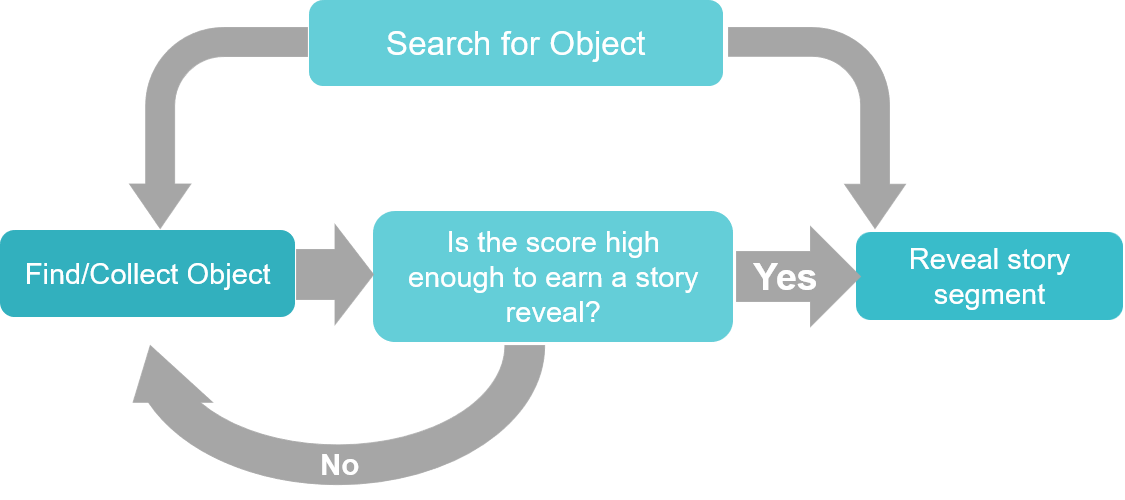
\includegraphics[width=2.5in]{imgs/Gameplay.png}
\caption{Description of the Gameplay}
\label{Gameplay}
\end{figure}

The story occurs in a science fiction setting that places the player in the role of an explorer. The player finds himself exploring ruins on another world that once housed an advanced civilization and is charged with learning how its members lived and what caused their disappearance. The player must then find objects, divided into three categories, that will divulge the necessary information about how this lost civilization lived and why it disappeared. Categories consist of Culture, Politics, and Technology and correspond to the nature of the player’s discoveries and tell the story of the civilization in tandem. For example, culture objects reveal how the civilization lived and what cultural tensions were present before they disappeared. Furthermore, the story arc of the civilization’s culture is told independently of the technology and politics story arcs, but with the common overarching plot of the civilization’s demise. An illustration of the story arc concept is presented below in \autoref{Tandem}. The first episode of the story can be found in \autoref{StoryPods Script Episode 1} of the appendix.

\begin{figure}[h]
\centering
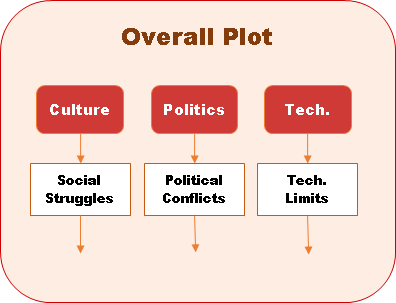
\includegraphics[width=2.5in]{imgs/TandemPlot2.png}
\caption{Illustration of Tandem Story Arcs}
\label{Tandem}
\end{figure}

Given the rules, mechanics, and the location-based nature of the game, some data and database design considerations are:

\begin{enumerate}
	\item Database requirements for working with geospatial data: It is necessary to understand data types, how they are stored, and how they may be obtained both from the player and by the player. 
	\item DBMS options: It is necessary to survey what database management systems and existing software packages are available that work well with GPS data and are also capable of storing the required tables and enforcing game rules.
	\item Database schema: It is imperative to know what entities and attributes must be stored and what relationships need to be enforced in order to develop the conceptual design for the database.
	\item Client side: In order to develop and test a prototype of the game, it is necessary to develop some kind of interface that interacts with the user and allows the user to play the game.
	\item Middle layer API: In addition to the client-side application, it is necessary develop some application that implements the player’s actions and interacts with the database accordingly.

\end{enumerate}

\subsection{Database requirements and selection}

We defined the database requirements as follows:

\begin{itemize}

\item The database must be able to store the player’s information, including player's ID, email, and other attributes.
\item The database must be able to store GPS location data. An important aspect when dealing with geospatial data is how to represent the data efficiently in order to reduce network traffic and storage requirements. A geospatial location is defined by its latitude and longitude coordinates. There are different formats in which these coordinates can be represented. The most common format for many applications (such as Google Maps and Geographical Information Systems or GIS) is the signed degrees format in which latitudes range from -90 to 90, and longitudes from -180 to 180.
\item The database can update the player's location. For the purpose of supporting the gameplay, it is important to update player’s locations when they move to a new destination where collectible objects are available. The database system must ensure the consistency and accuracy of the data even when the information of many closely-located players is been updated frequently. 
\item The location data must be stored with enough precision to support the actions of collecting objects. Latitude and longitude data are more precise when they use more decimals. Using 8 decimal places would give an exact location within 1 millimeter. This information is important because it determines, along with the number of players, how much data is stored in the database. If the amount is very large, some sort of data compression would be necessary.
\item The system must have a function to calculate scores for each player, adding the value of the collected objects. The system also records subtotals for each object category and recognizes when thresholds are reached, triggering new story segments.
\item The database must be able to interface with the AWS platform where the data is stored, and the middle layer API.

\end{itemize}

We assessed four database options:

\begin{enumerate}

\item \textbf{MySQL}. This database provides support for spatial data formats, functions for the required calculations of scores, and a purpose-built MySQL database for integration with AWS. Another advantage is the simplicity of its interface and widespread usage due to its open source nature. Some disadvantages include: no support for dedicated calculations with geospatial data (distances, surfaces, etc.), and limited Scalability in case there are requirements to support a large number of players. 

\item \textbf{PostgreSQL}. PostGIS is a spatial database extention for PostgreSQL. It adds support for geographic objects allowing location queries to be run in SQL. The three features that PostGIS delivers to PostgreSQL DBMS are spatial types, indexes and functions such as distance, area, union, intersection, and specialty geometry. AWS offers a purpose-built PostgreSQL database. Another advantage is that PostgreSQL is the recommended relational database for working with Python applications, which are a essential component of the middle layer.

\item \textbf{MongoDB}. MongoDB is a document database with an expressive query language, support for secondary indexes and easy accommodation of changes in applications. The dynamic document data model of MongoDB removes the need for a central catalog describing the structure of documents. Every document is self-describing by defining the field names internally, which comes at the cost of greater use of space. Data is stored in the BSON format, a binary encoding of JSON, which does not compress data. 
Regarding location data, MongoDB offers geospatial indexes, which allows location data to be efficiently retrieved based on longitude and latitude. Such an index is useful only if records contain other fields beside location. It also offers support for AWS. The main disadvantage is that the support of more complex documents makes it less simple than a SQL database. 
 
\item \textbf{Cassandra}. Another popular NoSQL database is Cassandra. According to our research, however, the development of geospatial data indexing and retrieval features has been lacking for this database.  Recent research show how geohashing techniques can be used to index store data, converting the latitude/longitude information to a numeric geohash attribute and associating it to the data when being stored. However, this might make this database less attractive than the other options. 

\end{enumerate}

Based on this assessment, we selected the open-sourced PostgreSQL database, integrating the capabilities of the PostGIS extension. Apart from the aforementioned advantages of using these tools, our research indicates that PostGIS is close to becoming the standard to manage geolocation data for SQL databases.  This allows us to build a database with the following capabilities:

\begin{itemize}
\item	Once the data is uploaded, use simple SQL language to run complex queries related locations, objects, and other spatial data. 
\item Scale out the database in various ways: manage a very large data size because it offers multi-TB capabilities, handle a large amount of concurrency from the data, use table-partitioning to break large data sets down into more manageable pieces.
\item Build custom functions using a language such as Python or R, which will be very useful to program the game requirements, rules and mechanisms into the database. 
\end{itemize}

\section{Description of the system}

\subsection{High-level system overview}
In order to be able to serve big number of requests in a timely manner and scale well with increasing number of players we need a system that will not only have a well designed, scalable database, but also other components integrated into a single, well thought architecture. Layout of all components of our system are represented schematically in \autoref{schema}.  Our system is built from 3 major parts:

\begin{enumerate}
  \item Client-side application: We decided to support 2 major platforms that got widespread adoption: Android and iOS. For the proof-of-concept we focused on iOS first. 
  \item Backend services, or middle layer: This component performs server-side operations, enforces gameplay rules and handles requests to our database. 
  \item Geospatially enabled database: Here all information regarding our players, objects and corresponding states is being kept. 
\end{enumerate}

We use following communication protocols between these components:

\begin{enumerate}[label=\Alph*]
\item REST over HTTP. This protocol is used to send messages from the client to the middle layer and back
\item SQL. We use relational database and SQL over Application Layer of the TCP/IP model to transform and query our data. 
\end{enumerate}

On the client side we have an iOS application that monitors longitude and latitude of a device and places objects around player. We calculate bearing, the horizontal angle between the direction of an object and player and distance between player and an object to place stories around given location. 

We want our backend to support large number of requests coming from multiple players. To achieve that we host our middle layer and our database on  Amazon Web Services (AWS).  We can use multiple copies of the identical service to scale our system up or down horizontally depending on the level of load.  To spread load across multiple copies of the service we can use AWS load balancer that distributes client’s requests in a round-robin fashion between instances. 

\begin{figure}[h]
\centering
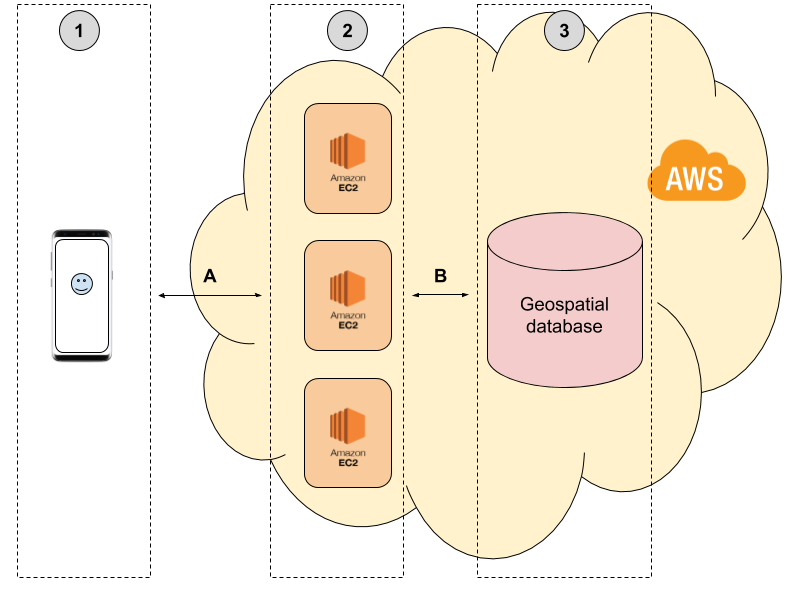
\includegraphics[width=2.5in]{imgs/systemschema.png}
\caption{Schematic layout of major components of the system}
\label{schema}
\end{figure}

\subsection{Database design to support the gameplay}

The important entities that the database must keep are: players, geospatial objects, stories and story-segments. We also need to know a player’s score in order to know what story segments the player has earned. Similarly, we need to know what objects have already been collected in order to not allow the player to collect them again. 

\begin{figure}[h]
\centering
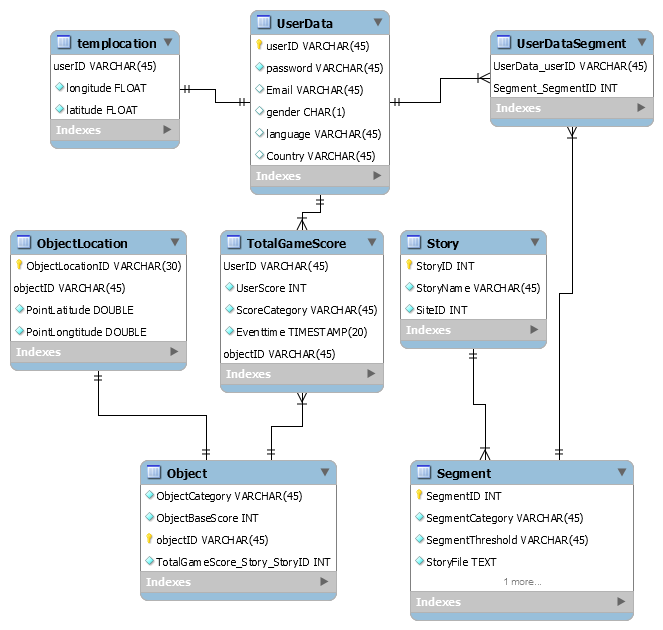
\includegraphics[width=2.8in]{imgs/DatabaseSchema.png}
\caption{Entity Relationship Diagram of StoryPods}
\label{ERD}
\end{figure}

A list of geospatial points that correspond to viable latitudes and longitudes that can be used for any particular game is stored separately from the list of geospatial points that are actually available to the player. This allows us to update the list and properties of physical geospatial points without affecting existing games and applications. A diagram of the database schema can be found in \autoref{ERD}. 

\subsubsection*{Players}
The UserData table contains ID and other attributes of all registered players taking part in the game. In the TempLocation table we store the player’s geographic location using the format provided by the PostGIS extension, which is a geographical point (latitude, longitude). We collect the player's location using the middle layer. We do not keep history of a player’s location.

\subsubsection*{Objects}
The Objects table includes a unique identifier (ObjectID), the object category (culture, economy or technology), and an attribute for the number of points awarded by each object (ObjectBAseScore). The game can run multiple stories, and therefore there’s a variety of objects that appear depending on the Story in which the player is immersed. This is why the StoryID attribute also appears on this table. 

The main mechanism of the game is collecting objects in different locations, which are described in the ObjectLocation table. The ObjectLocationID serves to record all the locations where objects can be collected. The latitude and longitude of the location are stored on this table, in order to match that information with the player’s location.

\subsubsection*{Scores} 
The database needs to keep the player’s score and link it to the UserID, and this is done in the TotalGameScore table. The table records the score by object category and adds up the total UserScore. 

\subsubsection*{Stories and Story Segments}
As players make progress through the game, collecting more objects and reaching predefined score thresholds, new segments of the story unfold until the player reaches the end. This information is stored in the Segment Table, which contains the SegmentID, the score Threshold that the user should achieve to unlock the segment, and a text StoryFile that is displayed on the device. 

The user will have several stories to choose from. These are stored in the Story table, which has a unique StoryID identifier along with the StoryName. 
Finally, in order to keep track of the User’s progress through the strory segments, by relating both entities in the UserDataSegment table. 

\subsection{Description of the middle layer}

We use Python to serve Application Program Interface (API) and PostGIS, a spatial database extension of PostgreSQL for spatial queries. Endpoints of the middle perform following important functions:

\textbf{Player Registration:} Record user profile data (UserID, name, email, address and etc) of the client. The data stores in database at "userdata" table.  Input is in JSON format 

\textbf{Player State Synchronization:} Provide summarized user score per category based on UserID as a response to the client request from the database. Response is in JSON format.

\textbf{Player location:} Instantaneously collect the player’s location data (latitude and longitude coordinates), and update this information in the database when the player moves according to the set thresholds (one update every 0.5 sec). The table has one record per user.

\textbf{List of Objects around the player’s location:} Send a response to the client reporting all objects available for collection, based on current position within a specified radius. Response is in JSON format.

\textbf{Collision report:} The middle layer stores a fact of a collision of a player with an object and responds with new player's score and reveals a new story segment. Input and Response is in JSON format.

\subsection{Client-side application}

A lot of work was done on the client side. For our prototype we’ve developed an iOS application only. The application does not interact with database directly and uses RESTful interface of the middle layer to read and manage any data. 
In \autoref{UserInterface} you can see schematic representation of the communication protocol that is used by the iOS application to support the gameplay. 
The application uses \textit{Synchronize Player’s State} endpoint to update user's data when the application starts or when a player changes any of his attributes. We use \textit{Apple's Vendor Identifier}\footnote[1]{Apple's Vendor ID: https://goo.gl/fGTV5g} to uniquely identify a player. 
Application uses \textit{Core Location Framework}\footnote[2]{Apple Core Location Framework: https://goo.gl/S83st9} to get longitude and latitude of a player approximately twice a second and reports it to the middle layer of our game via \textit{Report My Location} endpoint. 
Once location is known, iOS application requests all objects within 500 meters from player and uses \textit{ARKit}\footnote[3]{Apple ARKit Framework: https://developer.apple.com/arkit/} to place spheres around the player. When collision is detected by the application it reports it to the middle layer and our server sends back scores and a new segment if player's score is any category has reached segment's threshold.

\begin{figure}
\centering
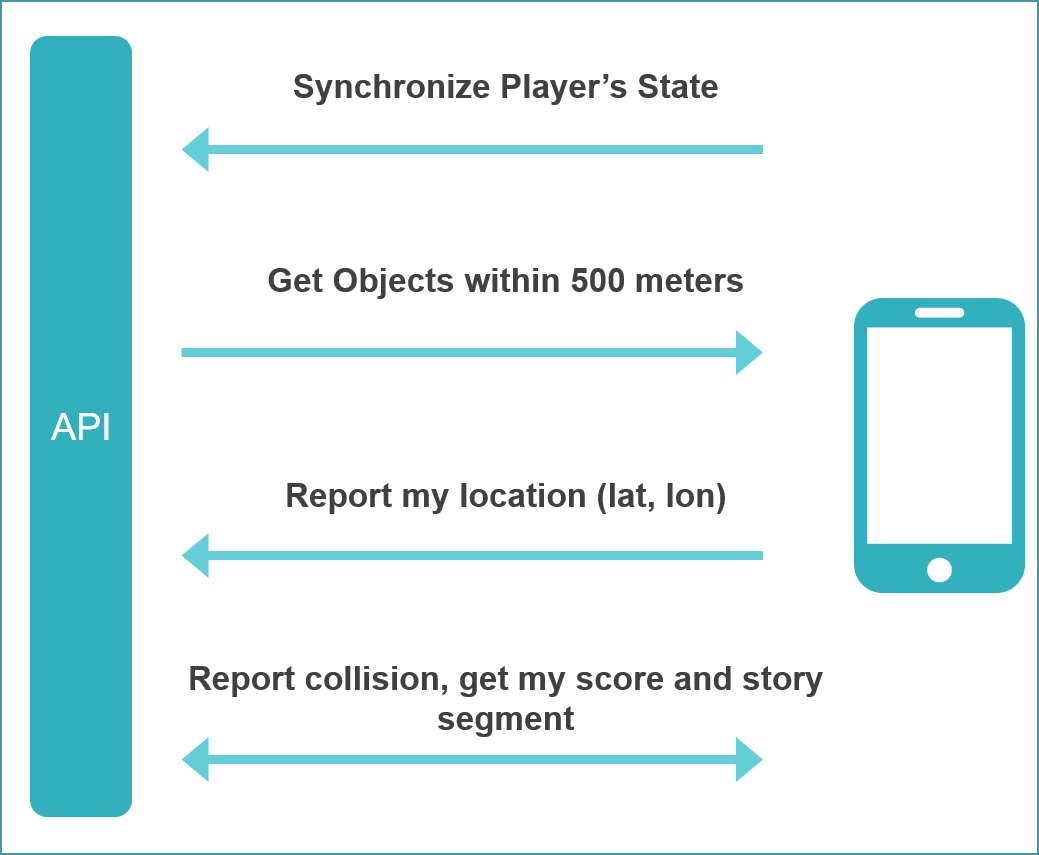
\includegraphics[width=2.5in]{imgs/UserInterface.png}
\caption{Diagram of User and Server Interfaces}
\label{UserInterface}
\end{figure}

\section*{Links to the game, code  and demonstration video}

We've shared a short video demonstrating our game in YouTube:

\begin{center}
\textit{\small{\url{https://goo.gl/xrNPXQ}}}. 
\end{center}

All the code, including presentation materials can be found in GitHub:

\begin{center}
\textit{\small{\url{https://github.com/VolodymyrOrlov/MSDS7330FinalProject}}}. 
\end{center}

Our application is not eligible for Apple Store since Apple does not allow prototypes to be shared with public. We use Apple’s TestFlight instead to share our game with anyone who wants to try it. To get our game on your device make sure your iPhone is 6s (model A1688) or higher and your iOS is updated to at least version 12.0.  Next, follow this link from your device to install Apple's TestFlight and our game: 

\begin{center}
\textit{\small{\url{https://testflight.apple.com/join/k9jZ6XeR}}}
\end{center}

\section{Conclusion}

While developing a prototype of a geospatially-enabled game we identified the following lessons and challenges:

\begin{enumerate}
\item Database and schema selection: there was no unique solution to meet the needs of our project. We found many options that offered different levels of performance, reliability, additional features.
\item Integration of APIs: We learned that the DBMS is just one element of the system. For the application to succeed we spent a large amount of time developing the middle layer.
\item Scalability: For the development of the prototype, the consideration of scalability was not very important. Our database selection would have changed if it was an immediate necessity. 
\end{enumerate}


\appendices

\section{StoryPods Script Episode 1}
\label{StoryPods Script Episode 1}

\subsection{Culture Line}

\subsubsection*{5 Points}
The abandoned city appears to have been well preserved due to its massive walls. This is excellent as it should also preserve all the dwellings, tools, art, and such within. No city of comparable size or as well preserved can be found anywhere near this place. In fact, the environment is so hostile that we would never have thought that this planet sustained life, much less complex civilizations. 

It is to think that not only were we able to find intelligent life but that we may be able to figure out how they lived. However, we must be wary that cultures that grow in isolation often fail to resemble the people and cultures everywhere else. Every preliminary conclusion must be taken with a grain of salt until we have more information. 

\subsubsection*{10 Points}
All the remains in the city appear to have the same aesthetic of jagged surfaces made from the same white material. Back on earth, cities tend to have vistas that vary according to the time they were constructed or the person who ordered their construction. Buildings, cars, lights, lampposts, and walkways all vary by when they were built or who was hired to build them. Most objects and buildings here look the same. Everything appears to have the same white and clean, if not Spartan look to them. This somewhat implies a single dominant culture, or at least that someone wants to make it look that way. After all, we don’t know if this is a genuine city that housed civilians or some kind of military or commercial outpost.  Perhaps this city had a purpose.

\subsubsection*{15 Points}
We have yet to find a single grave, or any kind of organic material, which is going to make it really difficult to learn about these beings’ biology and anatomy. It’s also going to be difficult to know exactly how many beings actually lived here at a time without some way to gauge birthrates, death rates or longevity. 

However, we must be wary not to blinded by earth bias. we don’t know if this implies longevity or perhaps a particular form of disposing of the dead, like cremation. We can’t even assume that the beings were a traditional form of life. We can only lament that they have all disappeared and have not even left remains for us to analyze. Hopefully, they left peacefully and voluntarily. 

\subsubsection*{20 Points}
Everything small enough to be picked up and held has a generally pleasant feel to it, at least by the standards on earth. Some of that could be the varying gravity, but this is also in spite of the larger size of everything. This craftsmanship present in our technological samples contrasts with the utter lack of public displays of art anywhere in the city. The ubiquity of the material implies that it has a utilitarian purpose, opposed to cultural or artistic one. Case in point, only military installations and penal colonies back on earth tend to have everything be the same color while having little to no unnecessary decorations. Going on first impressions: the beings appear to be far more motivated by utility and uniformity than by artistry and variety.

Then again, maybe their eyes work differently from ours. Maybe what they can see through their eyes is very different than what we can see through ours.  Let’s hope that this is indeed a peaceful, civilian outpost and that we are using our limited experience to assume too much. If it isn’t a civilian settlement, however, we are likely to get a very biased look at the beings’ culture. 

\subsubsection*{25 Points}
The team is waiting for permission to go underground and explore what may be beneath the city. We shouldn’t get our hopes up, as the request may not get approved and the city may not have much of an underground portion at all. In the chance that there were an underground portion of the city, we would have a second chance to find remains, waste, or some indicator of what food the inhabitants ate. There’s even a tiny possibility that someone is still alive but hiding beneath the city.

This is all an incredibly motivating prospect, since conclusions about how the beings lived have been incredibly limited without having decoded communiques. There are linguists, for example, who will be crucial in understanding the beings’ language but currently have very little to do. In the meantime, they can aid the xenoarchaeologists in a dig. Is there something they are afraid we are going to discover?

\subsection{Politics Line}

\subsubsection*{5 Points}
This is the only city of this size that can be seen anywhere on the planet. There is definitely evidence that there were other cities and settlements on this planet, but this is by far the biggest that we’ve been able to find. It’s also unusual by earth standards in that the largest cities on earth tend to be near water or on important trade routes. This city, however, is tucked away on arid steppes. The beings that built this city definitely went out of their way to isolate themselves from their environment, from valuable resources, and from others. As such, one would think that this should be one of the smaller cities on the planet. Since, nothing this big is ever built without a purpose. It makes me wonder just what the city is for.

\subsubsection*{10 Points}
No statues have survived. If there were statues or monuments, we could have gotten a sense of what or who the beings idolized. We might have even been able to know what the beings looked like. With no statues or monuments, however, we can’t necessarily conclude that they did not have any kings or idols. 

The city’s layout is also unusual in that there’s a doorway in the center. It’s a slanted doorway that just seems to lead into the ground. Ultrasounds confirm it doesn’t actually lead anywhere, which is really strange. On that note, ultrasounds also confirm that other parts of the city do have an underground network. So, we shouldn’t  jump to conclusions as we are just learning about this civilization, but a doorway that leads into directly into the ground at the center of the city is really unusual.

Also, it makes sense that a city confined by the walls has to get creative when expanding, but why did these beings choose to build down when they could have built up?

\subsubsection*{15 Points}
While the city has massive walls protecting it from without, it’s unusual to see a city of this size that has walls protecting it from the outside, but no second set of walls on the inside. Back on earth, most cities that feel threatened enough to build a set of giant walls, and have the technological and economic acumen to do so, rarely build just the one set. Come to think of it, once a certain amount of technological sophistication is achieved civilizations on earth tended to forget about walls and go with less visible and less intrusive but more sophisticated means of defense such as radar. As intruders, we should definitely be careful. Let’s hope the walls are just symbolic.

\subsubsection*{20 Points}
Those on the team who would like to study more complex topics like politics and culture have submitted a request to start exploring beneath the city. Mostly, that’s because nobody has been able to find an entry-way towards the underground and so some are suggesting creating one ourselves. Unfortunately, it is still not obvious what exactly is a door in this place, and even then, the city is still without power. Right now, we’re stuck sightseeing on the surface where there are no advertisements, or graffiti, or any attempts at mass public communication. Until we start receiving decoded and translated data, our best chance to study this place’s social dynamics is to have access to the actual dwellings, above or below ground.

P.S. It’s ironic to be lectured by engineers, who regularly learn about things by taking them apart, on the virtues of preserving the thing you are trying to understand.

\subsubsection*{25 Points}
Safety concerns are dominating the consideration for digging underground. While it appears that nobody else is here, we don’t know that to be true with 100\% certainty. Even if that may be true, we also don’t know if the city is still capable of communicating or transmitting information to anyone else. If it is, our intrusion has the possibility of being interpreted as an act of aggression. Given the fortress-like structure of the city and the mounting evidence that this could be some kind of military or penal colony, then our actions also have the potential to be construed as a declaration of war on behalf of all of humanity. 

However, the city/fortress being entirely deserted is still the most likely scenario. Also, the possibility of a miscommunication with other intelligent life in their sovereign space and the danger that comes with that should have been considered begore embarking on the mission at all, as this possibility is always present when communicating with intelligent life. If the leadership really believed we were in any immediate danger the we should be given orders to leave. Hopefully, that won’t turn out to be the case.  

\subsection{Technology Line}

\subsubsection*{5 Points}

We are inside the city’s walls now. We had to be airlifted into the center of the city because we couldn’t seem to find an entrance through the city’s enormous walls. Everything inside looks very advanced, though it’s hard to tell. We won’t know anything for sure until we bring objects back to the lab for analysis. Our instructions are to bring back anything that looks out of place so as to not upset evidence that may tell us how these beings lived. We have strict instructions, however, to not bring back any object that looks like an applicator, which means anything that looks like it’s meant to be pointed at something. Right now, we can’t tell the difference between a camera and a gun. As a safety rule: if it looks like it’s meant to be pointed at something then we should wait until we better understand this technology in general before we even begin to analyze it. 

\subsubsection*{10 Points}
Looks like binary is almost universal. Of what we’ve been able to bring back to the lab, most of what we’re studying operates on 1 or 0 transistors like on earth. There are some objects, however, that we can’t seem to make sense of but they do look like they would be useful. Case in point, the only thing we a screen that we brought back has a very parsimonious interior. It’s exciting to imagine what this advanced tech can teach us about computing, especially since it’s likely to be compatible with the ‘antiquated’ transistor technology from back home.

On a similar note, we haven’t been able to find anything that resembles a car or a ship. It makes you wonder how they got in or out.

\subsubsection*{15 Points}
Carbon dating shows that all of the objects that appear advanced are somewhat young. The objects that still rely on transistors, however, vary greatly in age. More precisely, the amount of C14 in the atmosphere is fairly high, but the older bits of tech have an unusually low C14 to C12 ratio. So, either the tech did not come from this planet with this atmosphere, or it was built a very long time ago, assuming atmospheres take a very long time to change. Is it possible that this civilization is like us and encountered an advanced civilization in the past? The tech being extraterrestrial would explain the substantial difference in C14 ratios. Of course, extinction via environmental destruction is still a possibility, but that would not be a very satisfying explanation as to why this is the only place left.

\subsubsection*{20 Points}
A few things are holding up our progress in analyzing the tech. We’re trying to first analyze the tech in some theoretically noninvasive way before trying taking it apart or physically altering it. We’ve tried millimeter scanners, electron spectroscopy, LiDAR, and hyperspectral imaging, but all of them are indicating that these objects are not even there. Billions of dollars in scanning and detection technology can’t seem to outdo the human eye, at least in proving that these objects exist. Additionally, everything in the city from the tallest buildings to hand held devices is covered in the same material. It’s possible the entire city is resistant to being electronically detected, which is all the more baffling given the lack of other signs of intelligent life on this planet. After all, why hide from electronic detection if there are no other electronics anywhere on the planet?

\subsubsection*{25 Points}
Thinking about it some more, if the city was designed to be undetectable by electronic scanning, then the ultrasounds are not going to be reliable. Ultrasounds have only been able to detect some empty spaces beneath the city that are very unlikely to be natural.  We have no way of knowing how much more of the city is below ground electronically. We would have to go below ground in person to know for sure. 

While many feel it would be prudent to wait until we understand the technology better, others are getting impatient with the slow progress in decoding the beings’ technology. The pretext of safety may be phony, however.  Having learned of the possibility of an underground component for any city, it’s logical that we intend to eventually explore the underground to learn as much as we can. It’s a question of when. So, it makes one wonder if the mission objective has changed now that we have found technology that can be incorporated into our  military back home. 


\begin{thebibliography}{1}
  
\bibitem{destination-engagement}
Koo Chulmo, Choi Kyuwon, Ham Juyeon, Chung Namho. Empirical Study About the PokémonGo Game and Destination Engagement, 2018

\bibitem{pokemon-motivation}
Marquet O, Alberico C, Adlakha D, Hipp JA. Examining motivations to play Pokemon Go and their influence on perceived
outcomes and physical activity. JMIR Serious Games 2017

\bibitem{location-based-mg}
L. Lehmann, Location-Based Mobile Games. GRIN Verlag Munich Germany, 2012.

\bibitem{data-store-issues}
J. Krumm and S. A. Shafer. Data store issues for location-based services. IEEE Data Eng. Bull., 2005.

\bibitem{location-based-services}
Jensen, C., Christensen, A., Pedersen, T., Pfoser, D.,Saltenis, S. and Tryfona, N. (2001). "Location-Based Services: A Database Perspective" Proceedings of Scandinavian GIS

\bibitem{massive-amounts-location-data}
K. Midtgård. Collecting massive amounts of location data in a NoSQL database. Master of Science in Computer Science, Norwegian University of Science and Technology, 2017

\bibitem{game-methodology}
R. Dillon, "The 6-11 Framework: A new methodology for game analysis and design" presented at the Proceedings Game-On Asia Conference, Singapore, Mar., 2011.

\bibitem{location-based-games}
L. Lehman, "Location-based Mobile Games" Technical University of Berlin, unpublished, 2012.

\bibitem {PostGIS scale}
Ramsey, Pau (2017)l. Scaling PostgreSQL and PostGIS, Dec 2017. URL: http://blog.cleverelephant.ca/2017/12/postgis-scaling.html

\end{thebibliography}


\end{document}
